\documentclass[10pt, spanish, twocolumn]{article}

% --- Paquetes de Diseño Editorial NYT ---
\usepackage[utf8]{inputenc}
\usepackage[T1]{fontenc}
\usepackage{babel}
\usepackage{amsmath, amssymb, amsfonts, amsthm}
\usepackage{libertinus} % Tipografía Serif clásica y elegante
\usepackage[default]{montserrat} % Sans-serif para headers modernos
\usepackage{microtype} % Perfección en el espaciado
\usepackage[margin=1.5cm, top=2.5cm, bottom=2cm, columnsep=0.8cm]{geometry}

% --- Paquetes para Gráficos Mega Profesionales ---
\usepackage{tikz}
\usepackage{pgfplots}
\pgfplotsset{compat=1.17}
\usetikzlibrary{shapes, arrows.meta, positioning, calc, backgrounds, patterns}
\usepackage{booktabs} % Tablas profesionales

% --- Paleta de Colores "The New York Times" ---
\usepackage{xcolor}
\definecolor{nytblack}{RGB}{18, 18, 18}
\definecolor{nytgray}{RGB}{120, 120, 120}
\definecolor{accentblue}{RGB}{50, 104, 145} % Azul de reportajes especiales
\definecolor{lightgray}{RGB}{240, 240, 240}

% --- Ingeniería de Títulos Estilo "Magazine" ---
\usepackage[explicit]{titlesec}
\titleformat{\section}
  {\normalfont\bfseries\sffamily\Large\color{nytblack}}
  {}{0pt}{\MakeUppercase{#1}}[{\color{nytblack}\titlerule[1.5pt]}]

\titleformat{\subsection}
  {\normalfont\bfseries\sffamily\normalsize\color{accentblue}}
  {}{0pt}{#1}

% --- Letra Capital Gigante ---
\usepackage{lettrine}
\renewcommand{\LettrineFontSpec}{\itshape\color{nytblack}}

% --- Caja de "The Daily Brief" y Definiciones ---
\usepackage[most]{tcolorbox}
\newtcolorbox{briefbox}[1]{
    enhanced,
    colback=white,
    colframe=nytblack!20,
    arc=0mm,
    boxrule=0.5pt,
    leftrule=3pt,
    fonttitle=\sffamily\bfseries\small,
    coltitle=nytblack,
    title=#1,
    attach title to upper,
    after title={ \textbar \ },
    drop fuzzy shadow
}

\newtcolorbox{formulabox}[1]{
    enhanced,
    colback=accentblue!5,
    colframe=accentblue,
    arc=2mm,
    boxrule=0pt,
    leftrule=2pt,
    fonttitle=\sffamily\bfseries\small\color{accentblue},
    title=#1,
    sharp corners=south
}

% --- Header Estilo Periódico ---
\usepackage{fancyhdr}
\pagestyle{fancy}
\fancyhf{}
\fancyhead[C]{\small\sffamily\textbf{THE SCIENCE TIMES} \quad \textbar \quad \textbf{ALLGEMEINE GRUNDLAGEN}}
\fancyfoot[L]{\tiny\sffamily Basado en Papula (2024) | Quintana Silva (UPTC)}
\fancyfoot[C]{\thepage}
\renewcommand{\headrulewidth}{0.8pt}

\begin{document}

% --- Portada de Sección Mega Increíble ---
\twocolumn[
  \begin{center}
    \vspace*{-1cm}
    {\fontsize{50}{55}\selectfont\textbf{Matemáticas Superiores}} \\
    \vspace{0.2cm}
    {\fontsize{20}{22}\selectfont\textit{De la Teoría de Conjuntos a la Resolución de Ecuaciones Complejas}} \\
    \vspace{0.6cm}
    \begin{minipage}{0.9\textwidth}
        \centering
        \hrule height 1.2pt \vspace{2pt} \hrule height 0.5pt
        \vspace{0.1cm}
        \small\sffamily \textbf{DEEP DIVE} \quad $\bullet$ \quad FUNDAMENTOS CIENTÍFICO-TÉCNICOS \quad $\bullet$ \quad ENE. 2026
        \vspace{0.1cm}
        \hrule height 0.5pt \vspace{2pt} \hrule height 1.2pt
    \end{minipage}
    \vspace{0.8cm}
  \end{center}
]

% --- Inicio del Texto ---
\lettrine[lines=3, findent=2pt, nindent=0pt]{L}{a} transición del pensamiento escolar a la estructura de las disciplinas científicas superiores requiere más que fórmulas; exige un marco lógico. En este volumen, exploramos los cimientos del \textit{Allgemeine Grundlagen}: desde el átomo de la lógica en la teoría de conjuntos hasta la robustez de los sistemas de ecuaciones que modelan la realidad física.

\section{El Álgebra de los Conjuntos}

Las operaciones entre conjuntos (\textit{Mengenoperationen}) son el andamiaje del álgebra moderna. Permiten combinar entidades abstractas para definir nuevas unidades lógicas. Esta tríada de operaciones es fundamental para la ingeniería de datos y el cálculo.

\subsection{Intersección (Schnittmenge)}
La intersección $A \cap B$ es el crisol donde coinciden dos mundos. Se define como el conjunto de elementos que pertenecen \textbf{simultáneamente} a ambos conjuntos.
\[ A \cap B = \{x \mid x \in A \wedge x \in B\} \]
\textit{Ejemplo:} La solución de un sistema de inecuaciones es la intersección de sus conjuntos de solución individuales.

\subsection{Unión (Vereinigungsmenge)}
La unión $A \cup B$ representa la totalidad. Abarca todo elemento que pertenece a $A$, a $B$, o a ambos. Es un concepto inclusivo, fundamental en la probabilidad y la lógica digital.

\subsection{Diferencia (Differenzmenge)}
A menudo, lo que importa es lo que \textit{sobra}. La diferencia $A \setminus B$ (leído "A menos B") contiene los elementos de A que no están en B. Es la operación base para definir los números naturales positivos: $\mathbb{N}^* = \mathbb{N} \setminus \{0\}$.

\vspace{0.5cm}
\begin{center}
\textbf{\footnotesize FIGURA 1. VISUALIZACIÓN VENN DE OPERACIONES}
\vspace{0.3cm}

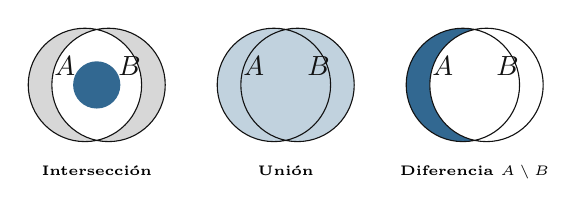
\begin{tikzpicture}[scale=0.6]
    % Intersección
    \begin{scope}[shift={(0,0)}]
        \fill[nytgray!30, even odd rule] (0,0) circle (1.2cm) (0.5,0) circle (1.2cm);
        \fill[accentblue] (0.25,0) circle (0.5cm); % Intersección destacada
        \draw[nytblack] (0,0) circle (1.2cm) node[above left] {$A$} (0.5,0) circle (1.2cm) node[above right] {$B$};
        \node[below] at (0.25,-1.5) {\tiny \textbf{Intersección}};
    \end{scope}
    
    % Unión
    \begin{scope}[shift={(4,0)}]
        \fill[accentblue!30] (0,0) circle (1.2cm) (0.5,0) circle (1.2cm);
        \draw[nytblack] (0,0) circle (1.2cm) node[above left] {$A$} (0.5,0) circle (1.2cm) node[above right] {$B$};
        \node[below] at (0.25,-1.5) {\tiny \textbf{Unión}};
    \end{scope}

    % Diferencia
    \begin{scope}[shift={(8,0)}]
        \begin{scope}
            \clip (0,0) circle (1.2cm);
            \fill[accentblue] (0,0) circle (1.2cm);
            \fill[white] (0.5,0) circle (1.2cm);
        \end{scope}
        \draw[nytblack] (0,0) circle (1.2cm) node[above left] {$A$} (0.5,0) circle (1.2cm) node[above right] {$B$};
        \node[below] at (0.25,-1.5) {\tiny \textbf{Diferencia $A \setminus B$}};
    \end{scope}
\end{tikzpicture}
\end{center}

\section{Reales: La Estructura del Continuo}

Los números reales ($\mathbb{R}$) no son solo símbolos; son la correspondencia biunívoca con los puntos de una recta geométrica. Incluyen finitos, infinitos periódicos y, crucialmente, los irracionales.

\begin{formulabox}{LEYES ESTRUCTURALES}
El cálculo en $\mathbb{R}$ se sostiene sobre pilares inquebrantables:
\begin{itemize}
    \item \textbf{Conmutativa:} $a + b = b + a$ (El orden no altera la suma).
    \item \textbf{Asociativa:} $a(bc) = (ab)c$ (La agrupación es flexible).
    \item \textbf{Distributiva:} $a(b + c) = ab + ac$ (El puente entre suma y producto).
\end{itemize}
\end{formulabox}

\subsection{Orden y Valor Absoluto}
La recta numérica orienta la existencia. La relación $a < b$ tiene significado geométrico directo: $a$ está a la izquierda de $b$. 

El \textbf{valor absoluto} $|a|$ redefine el concepto de cantidad al eliminar la dirección: es la distancia al origen.
\[ |a| = \begin{cases} a & \text{si } a \ge 0 \\ -a & \text{si } a < 0 \end{cases} \]
Gráficamente, $y = |x|$ transforma negatividad en positividad, reflejando el eje inferior hacia el superior.

\vspace{0.3cm}
\begin{center}
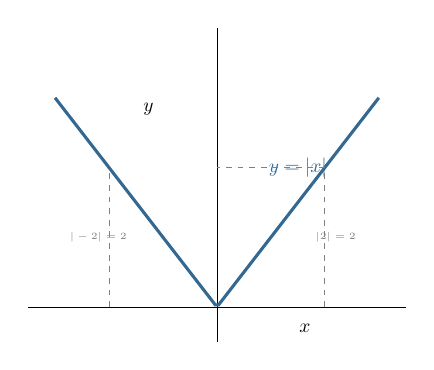
\begin{tikzpicture}[scale=0.7]
    \begin{axis}[
        axis lines=middle,
        xmin=-3.5, xmax=3.5,
        ymin=-0.5, ymax=4,
        xlabel=$x$, ylabel=$y$,
        ticks=none,
        axis line style={-},
        every axis x label/.style={at={(current axis.right of origin)},anchor=north west},
        every axis y label/.style={at={(current axis.above origin)},anchor=south east}
    ]
    \addplot[color=accentblue, ultra thick, domain=-3:3, samples=100] {abs(x)};
    \node[color=accentblue] at (axis cs: 1.5, 2) {$y=|x|$};
    \draw[dashed, gray] (axis cs: 2,0) -- (axis cs: 2,2) -- (axis cs: 0,2);
    \node[gray, font=\tiny] at (axis cs: 2.2, 1) {$|2|=2$};
    \draw[dashed, gray] (axis cs: -2,0) -- (axis cs: -2,2);
    \node[gray, font=\tiny] at (axis cs: -2.2, 1) {$|-2|=2$};
    \end{axis}
\end{tikzpicture}
\\ \footnotesize \textbf{FIG 2.} Simetría de la función valor absoluto.
\end{center}

\section{El Arte de Resolver Ecuaciones}

Una ecuación es una proposición de igualdad que desafía al analista a encontrar la incógnita. La dificultad varía desde lo lineal hasta lo trascendental.

\subsection{Lineales y Cuadráticas}
La ecuación lineal $ax + b = 0$ posee una solución única. La cuadrática $ax^2 + bx + c = 0$ introduce el misterio del \textbf{discriminante} $D$.
Si $D > 0$, dos soluciones reales; si $D = 0$, una solución doble; si $D < 0$, el resultado escapa a lo real hacia los números complejos.

\subsection{Desafíos de Grado Superior}
Las ecuaciones cúbicas y bicuadradas requieren artificios algebraicos como la sustitución $u = x^2$ o el esquema de Horner. Para sistemas de ecuaciones lineales ($A\vec{x} = \vec{c}$), el algoritmo de Gauss transforma el caos en un sistema escalonado, revelando si la solución es única, infinita o inexistente.

\begin{briefbox}{ADVERTENCIA LÓGICA}
Al resolver \textbf{ecuaciones irracionales} (con raíces), elevar al cuadrado ambos lados genera una transformación \textit{no equivalente}. Es obligatorio verificar los resultados para descartar soluciones falsas (\textit{Scheinlösungen}).
\end{briefbox}

\subsection{El Método Numérico: Newton}
Cuando el álgebra se rinde, la computación avanza. El método de Newton (*Tangentenverfahren*) aproxima raíces mediante iteraciones geométricas usando tangentes a la curva.

\vspace{0.2cm}
\begin{center}
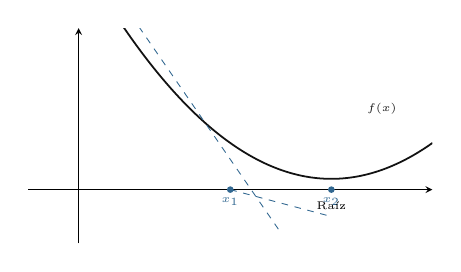
\begin{tikzpicture}[scale=0.8]
    \begin{axis}[
        axis lines=middle,
        xmin=-0.5, xmax=3.5,
        ymin=-1, ymax=3,
        ticks=none,
        width=8cm, height=5cm
    ]
        % Función ejemplo
        \addplot[color=nytblack, thick, domain=0:3.5, samples=100] {(x-2.5)^2/1.5 + 0.2};
        \node[font=\tiny, color=nytblack] at (axis cs: 3, 1.5) {$f(x)$};
        
        % Tangente 1
        \draw[dashed, accentblue] (axis cs: 0, 4.65) -- (axis cs: 2, -0.8);
        \fill[accentblue] (axis cs: 0, 4.65) circle (1.5pt) node[above left, font=\tiny] {$x_0$};
        \fill[accentblue] (axis cs: 1.5, 0) circle (1.5pt) node[below, font=\tiny] {$x_1$};
        
        % Tangente 2 (simulada)
        \draw[dashed, accentblue] (axis cs: 1.5, 0) -- (axis cs: 2.5, -0.5);
        \fill[accentblue] (axis cs: 2.5, 0) circle (1.5pt) node[below, font=\tiny] {$x_2$};
        
        % Raíz real aproximada
        \node[font=\tiny] at (axis cs: 2.5, -0.3) {Raíz};
    \end{axis}
\end{tikzpicture}
\\ \vspace{0.1cm}
\footnotesize\sffamily \textbf{FIG 3.} Aproximación sucesiva de Newton.
\end{center}

\vspace{1cm}
\hrule
\vspace{0.5cm}

\begin{tcolorbox}[enhanced, colback=nytgray!5, colframe=nytgray, title=\sffamily\bfseries\small SOBRE EL AUTOR, fonttitle=white]
    \begin{minipage}{0.2\textwidth}
        % Placeholder para foto
        \centering
        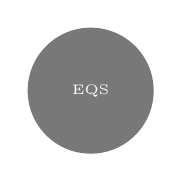
\begin{tikzpicture}
            \fill[nytgray] (0,0) circle (0.8cm);
            \node[white, font=\tiny] at (0,0) {EQS};
        \end{tikzpicture}
    \end{minipage}
    \hfill
    \begin{minipage}{0.75\textwidth}
        \textbf{Emanuel Quintana Silva} \\
        \footnotesize Economista en formación (UPTC) con gran pasión por la Econometría Computacional y la aplicación de \textbf{R} y \textbf{Python} en las Ciencias Sociales. \\
        \vspace{0.2cm}
        \footnotesize \textit{ORCID:} 0009-0006-8419-2805 \\
        \footnotesize \textit{Email:} emanuel.quintana@uptc.edu.co
    \end{minipage}
\end{tcolorbox}

\vspace{0.5cm}
\begin{center}
    \tiny\sffamily \textbf{REFERENCIAS BIBLIOGRÁFICAS} \\
    Papula, L. (2024). \textit{Mathematik für Ingenieure und Naturwissenschaftler Band 1} (16.ª ed.). Springer Vieweg. \\
    DOI: 10.1007/978-3-658-45802-7. ISBN 978-3-658-45801-0.
\end{center}

\end{document}